\chapter{Background}

Alle wichtigen Teile die nötig sind um die Arbeit im Detail zu verstehen werden im Folgenden erläutert. 

\section{Brain decoding and image reconstruction}


% \cite{grill-spectorHUMANVISUALCORTEX2004} Es ist schon lange bekannt, dass es im visuellen System Neurone gibt, welche von unterschiedlichen Reizen (zum Beispiel der Ausrichtung) von Objekten reagieren. Mithilfe von fMRI können die Regionen auch noninvasiv genauer untersucht werden. Zwei Hauptprinzipien: hierarchische Verarbeitung und funktionale Spezialisierung. 
% Hierarchisch, dass von V1 bis V4 immer komplexere Merkmale encoded werden. 
% Spezialisierung, verschiedene Wege die das where oder what pathway (also parallele hierarchische Sequenzen). 
% \cite{kourtziCorticalRegionsInvolved2000} Regionen, welche auf unterschiedliche Formen reagieren
% \cite{kanwisherFusiformFaceArea1997} die FFA, die vor allem auf Gesichter reagiert
% \cite{epsteinCorticalRepresentationLocal1998} die PPA, die auf Szenen reagiert aber nur wenig auf einzelne Objekte und gar nicht auf Gesichter. 

% Das Problem an dem ganzen ist, dass die Gehirne unterschiedlich funktionieren. Viel Forschung ist bezogen auf einzelne Regionen im Gehirn (wo also die V1 generell ist). Um genauere Informationen über die Stimuli zu erlangen ist es aber nötig, feinere Unterschiede zu treffen. Vom region based zu so fein granular based wie möglich (was bei fmri studien voxel sind).

% All das sind allgemeine Studien, welche das Encoding untersucht haben (also, wie sind Informationen im Kopf gespeichert). Es gibt den Unterschied zum Decoding \cite{naselarisEncodingDecodingFMRI2011}
% Encoding uses stimuli to predict brain activity, decoding uses brain activity to predict features of the stimulus. Both of them can be used for different usecases. In our study we want to reconstruct visual stimuli, thus we need to use decoding models. These are usually done with linear classifiers (because it's easy to train those with limited training data.) In the brain, there could be nonlinear interactions however, where the activation of voxels might be interdependent. Training classifiers that would uncover these would however need lots of data. 

% Decoding haben kamitani und Tong gemacht. \cite{kamitaniDecodingVisualSubjective2005} Es wurde mit fmri Aktivität im frühen visuellen System die orientation aus 8 möglichkeiten von edges vorhergesagt. Auch wenn die orientation columns wahrscheinlich kleiner sind, als die voxel, kann durch ensemble approaches doch die Information rausgelesen werden. Dabei waren für die orientation selectivity insbesondere Neurone in V1 und V2 wichtig. 


% \cite{miyawakiVisualImageReconstruction2008} machen einen ersten Schrit in die Richtung von genereller Bildrekonstruktion, bei dem Muster in 10x10 patches (also 2 hoch 100 mögliche States) gut vorhergesagt werden können. Dieses Paper geht also einen Schritt über reine Klassifikation hinaus. Einzelne lokale Decoder werden trainiert, die jeweils Teile des Gesamtbildes beschreiben können. Somit kann auch mit wenigen Trainingssamples schon eine hohe Generalisierung erreicht werden. Auch hier wurde noch mehr low-level information aus V1 und V2 gearbeitet. Informationen von höheren Regionen wie V3 und V4 hatten in diesem Modell noch keinen großen impact (v1 hatte die meisten Voxel die significant waren).


% Das Problem dass aus dieser Forschung folgte, war dass nur low-level Information aus den frühen Regionen genutzt werden konnte, damit also möglich ist zu rekonstruieren, wie die Umrisse von etwas aussehen, aber kein Inhalt über die semantische Bedeutung decoded wird. Horikawa Et al nutzen also einen Ansatz um higher level Regions auch in das decoding einzubinden und dabei nicht auf Klassifizierung angewiesen zu sein, sondern bestenfalls einen generellen Decoder zu erstellen. Deshalb verfolgen sie einen zero-shot Ansatz mit dem sie generic object decoding betreiben (dabei können beliebige objektkategorien aus der Gehirnaktivität gelesen werden). Mithilfe von sparse linear regression haben sie die feature vectors von CNNs unterschiedlicher layer vorhergesagt. Sie konnten zeigen, dass die hierarchische Verarbeitung im Gehirn auch auf die hierarchische Verarbeitung in einem CNN abgebildet werden kann. So können mit der Aktivität in tiefen Gehirnregionen (wie V1, V2) die low-level Features eines CNN vorhergesagt werden und mit hohen Gehirnregionen (V4, LOC, PPA, FFA) die high-level Features vom CNN. 
% \cite{horikawaGenericDecodingSeen2017}
 

It has long been known that the visual system contains neurons that respond to various stimuli, such as object orientation, movement or color~\cite{grill-spectorHUMANVISUALCORTEX2004}. Functional magnetic resonance imaging (fMRI) has enabled noninvasive examination of these neural regions in greater detail. The visual cortex follows two main principles: hierarchical processing and functional specialization. Hierarchical processing indicates that increasingly complex features are encoded progressively from primary visual area V1 up to area V4. Functional specialization refers to parallel hierarchical pathways, commonly known as the `where' and `what' pathways, which process spatial information and object identification, respectively~\cite{grill-spectorHUMANVISUALCORTEX2004}. Specific regions within the cortex have been identified to respond preferentially to different stimulus types; for instance, the fusiform face area (FFA) is specialized for faces~\cite{kanwisherFusiformFaceArea1997}, whereas the parahippocampal place area (PPA) predominantly responds to scenes rather than individual objects or faces~\cite{epsteinCorticalRepresentationLocal1998}. Further, cortical regions responding specifically to shape features have also been described~\cite{kourtziCorticalRegionsInvolved2000}. However, a key challenge arises from individual differences in brain organization and function. Many studies focus on broad cortical modules (e.g. V1), but detailed insights into stimuli (e.g. the region within v1 that codes for horizontal edges) require finer resolution. In order get a more granular view on brain regions, the voxels that the fmri measures can be analysed. Although the voxel size is still not granular enough to find single neurons that code for example for a specific orientation of stimuli, the `average' activation of the neurons within a voxel might lean towards a specific orientation of a seen stimulus~\cite{kamitaniDecodingVisualSubjective2005} and thus the voxels can contain this very granular information in an indirect way. When investigating brain regions, one can differentiate between encoding and decoding models. Encoding models try to predict brain activity depending on a given stimulus, decoding does the exact opposite: depending on measured brain activity, characteristics of a stimulus are supposed to be predicted~\cite{naselarisEncodingDecodingFMRI2011}. For reconstructing visual stimuli from measured brain activity, decoding models are essential. Decoding models typically employ linear classifiers due to their effectiveness in cases where the amount of data is limited. Although neural interactions within the brain may be nonlinear, revealing these interdependencies through more complex models requires extensive datasets, which is usually not feasible in fMRI experiments (both due to the high recording effort and the granularity of the recorded data). Early influential decoding work by Kamitani and Tong~\cite{kamitaniDecodingVisualSubjective2005} demonstrated that the orientation of edges (from eight possible orientations) could be predicted from fMRI activity from the activity early visual areas (V1 and V2). Despite orientation columns in the visual areas likely being smaller than individual voxels, ensemble decoding methods successfully extracted meaningful orientation information, that enabled the prediction of the orientation of seen stimuli. Advancing further, Miyawaki et al.~\cite{miyawakiVisualImageReconstruction2008} introduced a method for image reconstruction, successfully predicting visual patterns composed of 10$\times$10 pixel patches (resulting in $2^{100}$ possible states). They trained multiple local translators with slightly different features (for example single pixels or $2\time1$ pixel rectangles) that were then used together in an ensemble approach to reconstruct the shown stimuli. Like previous studies, Miyawaki et al.~ predominantly relied on low-level visual information from V1 and V2, as higher-level areas (V3 and V4) had minimal influence on the reconstruction. 
A limitation arising from this body of work is the predominant use of low-level visual information from early cortical regions, thus restricting reconstructions primarily to low-level features (like contours and textures) without capturing much of the semantic meaning. Addressing this limitation, Horikawa et al.~\cite{horikawaGenericDecodingSeen2017} developed an approach that was able to incorporate the influence of higher cortical regions into the translator. They were able to create a generic object translator, which enabled the prediction of diverse object categories from brain activity without relying on having a definite set of objects that was learned in the training data. Using sparse linear regression, they predicted feature vectors from different layers of convolutional neural networks (CNNs). This approach demonstrated a correspondence between the hierarchical processing within the human brain and CNN hierarchies: low-level CNN features were predicted from early visual regions (V1, V2), whereas high-level CNN features correlated with activity in higher visual regions (V4, LOC, PPA, FFA).

Now that features of deep learning models, it is possible to integrate higher brain structures into the decoding process. In this way, a general reconstruction of visual stimuli can be pursued, which is not only based on low-level image features, but also, for example, on semantically semantic categories (e.g.\ in~\cite{shenDeepImageReconstruction2019,ozcelikNaturalSceneReconstruction2023}). Shirakawa et al.~\cite{shirakawaSpuriousReconstructionBrain2024} describe the general workflow used by modern reconstruction algorithms. This pipeline is illustrated in Figure~\ref{fig:recon_pipeline}. Image Reconstruction essentially consists of two steps: first, a decoder is used to map the brain data onto latent features. \rOne{The word decoder is however used for many different concepts. Thus in this work, the model that translates the brain activity to some latent space will be called translator instead}. These latent features may, as in Horikawa et al.~\cite{horikawaGenericDecodingSeen2017}, contain aggregated information about the low-level and high-level visual information. Typically, a linear model is used for the translator, which can learn to predict the features robustly and with little data from brain activity. The latent features are then converted into an image in a second step using a generator module, which can use different techniques such as diffusion models~\cite{xuVersatileDiffusionText2024,ozcelikNaturalSceneReconstruction2023} or generative adversarial networks (GANs). These generative models are usually too complex to be trained with the small amount of recorded brain activity. Therefore, pre-trained models are used here to generate images from the previously predicted latent features.

\begin{figure}[ht]
    \centering
    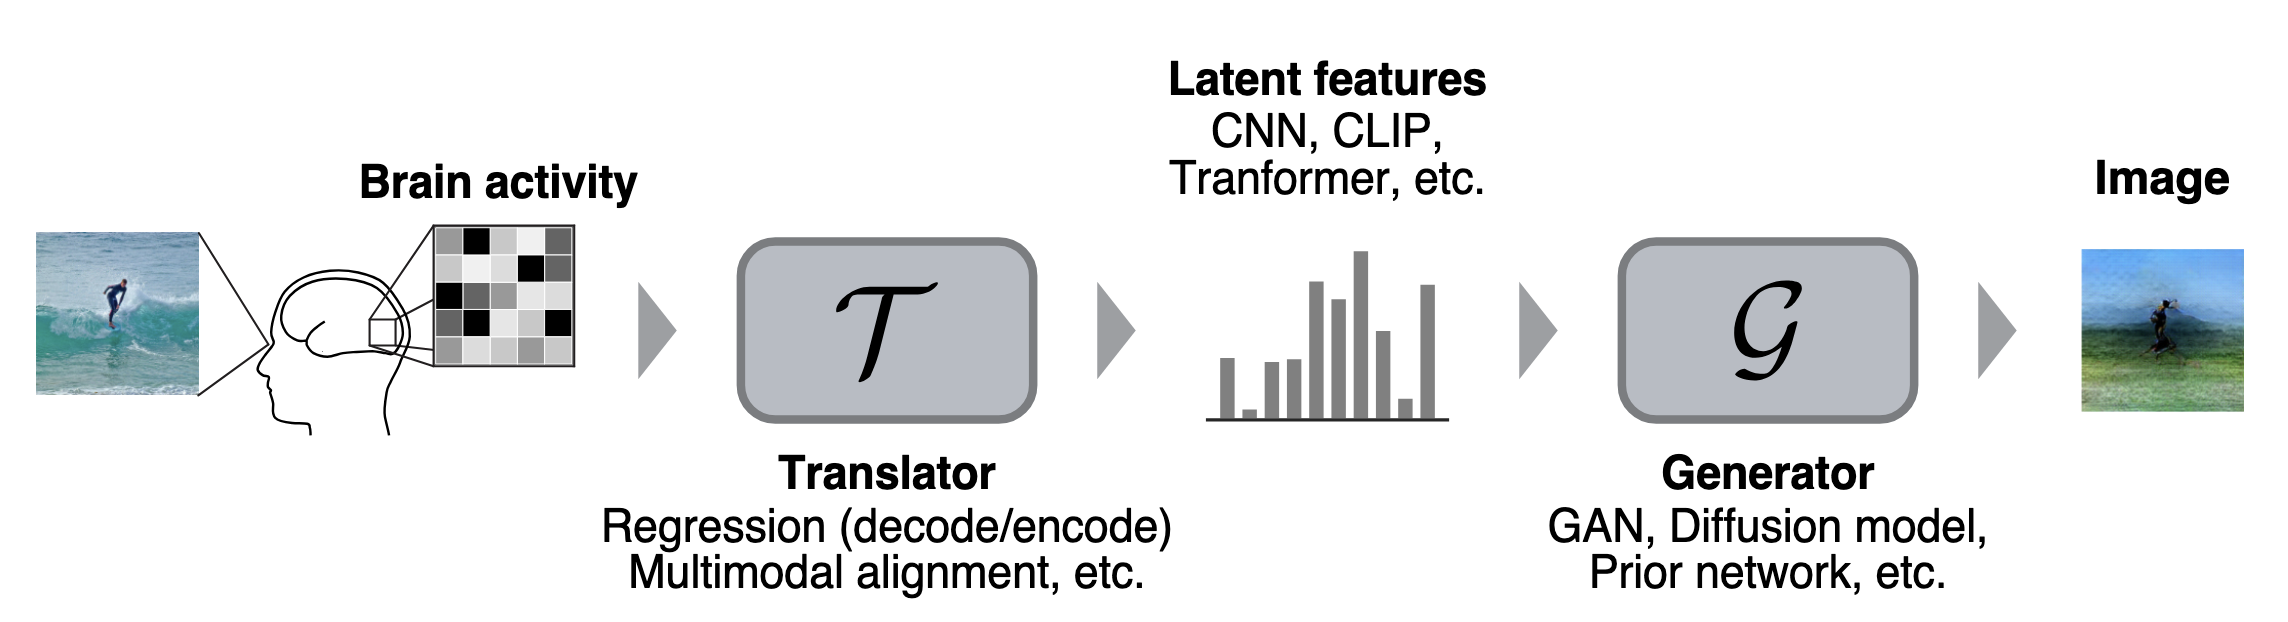
\includegraphics[width=0.8\textwidth]{plots/01_background_shirakawa_recon_pipeline.png}
    \caption[General Reconstruction Pipeline]{Visualization of the general Reconstruction Pipeline taken from Shirakawa et al.~\cite{shirakawaSpuriousReconstructionBrain2024}}\label{fig:recon_pipeline}
\end{figure}

One algorithm using this approach is the iterative Convolutional Network algorithm (iCNN), first described by Shen et al.~\cite{shenDeepImageReconstruction2019}. They adopted the method introduced by Horikawa et al.~\cite{horikawaGenericDecodingSeen2017} to predict hierarchical features of a deep neural network based on brain activity and subsequently used these features to reconstruct images that the participants have seen. Specifically, Shen et al.\ used a VGG-19 network that was pre-trained on ImageNet, to obtain features from the training images. Then a sparse linear regression was trained to predict these features from the brain activity. Then, for two different test datasets, the trained \rOne{translator} predicted the test features from the brain activity. Backpropagation is used to adjust the pixels in multiple steps to minimise the loss between the predicted features and the features, that the pixels produce in the vgg-19 network. In addition, an optional deep generator network was introduced to act as an image prior to improve the naturalness of the reconstructed images. Using this approach, Shen et al.\ successfully reconstructed both natural and artificially generated test images, effectively exploiting information from higher cortical structures. The iCNN has been used successfully to study the influence of attention on ambiguous stimuli. Horikawa et al.~\cite{horikawaAttentionModulatesNeural2022} showed two superimposed images in an experiment. Subjects were asked to focus on one of the images, and the image on which attention was focused could be successfully reconstructed. This shows that the iCNN can also be used to map attention-modulated top-down processes and does not only depend on the actual visual properties of an image. Cheng et al.~\cite{chengReconstructingVisualIllusory2023} used images that created optical illusions so that people perceived lines that were not actually present. These perceived (non-existent) features of the images could also be successfully reconstructed using the algorithm.




% Neben dem iCNN, welcher die Rekonstruktion über eine iterative Anpassung im Pixel Space vornimmt, gibt es noch eine zweite Gruppe an Rekonstruktionsalgorithmen, welche die Rekonstruktion über diffusion basierte Image creation durchführen~\cite{takagiHighResolutionImageReconstruction,ozcelikNaturalSceneReconstruction2023, scottiMindEye2SharedSubjectModels2024}. In der Regel wird auch bei diesen Algorithmen zunächst die Gehirnaktivität mit einem translator Modell (zum Beispiel lineare Regression) in einen latenten Feature space überführt. Diese latenten Features werden dann von einem vortrainierten diffusion model in Bilder umgewandelt. Der Brain-Diffuser Algorithmus wurde von Ozcelik et al.~\cite{ozcelikNaturalSceneReconstruction2023} entworfen. Der Brain-Diffuser nutzt drei verschiedene translator Modelle und übersetzt somit zunächst die Gehirnaktivität in drei verschiedene Feature Spaces: einerseits werden die latenten features eines very deep variational autoencoder (VDVAE) \cite{childVeryDeepVAEs2020} vorhergesagt. Der VDVAE kann dann genutzt werden um das Bild (allerdings mit wenig Details) zu rekonstruieren. Um zu dem Bild dann weitere Details hinzufügen zu können werden noch zwei weitere translator trainiert: einer, welcher die CLIP Vision~\cite{radfordLearningTransferableVisual2021} features der Trainingsbilder vorhersagt und einer, welcher CLIP Text features von captions der Trainingsbilder vorhersagt. Mithilfe der CLIP features sollen semantische Informationen und weitere Details aus der Gehirnaktivität extrahiert werden. Alle drei translator werden durch lineare ridge regression realisiert~\cite{hoerlRidgeRegressionBiased1970}. Nach dem die Gehirnaktivität in die drei feature spaces übersetzt wurden, werden diese genutzt um mit dem versatile diffusion Algorithmus~\cite{xuVersatileDiffusionText2024} die finale Bildrekonstruktion zu erzeugen. Bei der versatile diffusion wird dann in einem image to image Bildrekonstruktionsprozess zunächst die Rekonstruktion des VDVAE als Basis genommen und dann ein diffusion Prozess durchgeführt, welcher durch CLIP Vision und CLIP Text features konditioniert wird. Auf diese Weise kann der Brain-Diffuser die low-level features (Form und Farben) mithilfe des VDVAE rekonstruieren und dann durch die versatile diffusion mit den CLIP Vision und CLIP Text features anreichern, sodass ein natürlich aussehendes Bild generiert werden kann. Ozcelik et al. konnten mit diesem Algorithmus anhand des Natural Scense Dataset (NSD)~\cite{allenMassive7TFMRI2022} zeigen, dass das mehrstufige Verfahren dazu in der Lage ist, sowohl low-level als auch semantische high-level Informationen präzise aus der Gehirnaktivität zu extrahieren und die Bilder, welche den Probanden gezeigt wurden, erfolgreich zu rekonstruieren. 

In addition to the iCNN, which reconstructs images through iterative pixel-space adaptation, a second class of algorithms relies on diffusion-based image generation~\cite{takagiHighResolutionImageReconstruction,ozcelikNaturalSceneReconstruction2023,scottiMindEye2SharedSubjectModels2024}. Typically, these methods also first map brain activity into a latent feature space using translation models like linear regression. Subsequently, a pre-trained diffusion model generates the images from these latent features. The Brain-Diffuser algorithm by Ozcelik et al.~\cite{ozcelikNaturalSceneReconstruction2023} uses three linear ridge regression-based~\cite{hoerlRidgeRegressionBiased1970} translators, each converting brain activity into distinct feature spaces: latent features from a Very Deep Variational Autoencoder (VDVAE)\cite{childVeryDeepVAEs2020},  CLIP Vision features and CLIP Text features~\cite{radfordLearningTransferableVisual2021}. Initially, the VDVAE is used to reconstruct the basic image structure with limited detail. Subsequently, the CLIP Text and CLIP Vision features enhance the image by adding semantic and visual details. These three types of features are used to guide the versatile diffusion algorithm~\cite{xuVersatileDiffusionText2024}, which first uses the initially reconstructed VDVAE image as a baseline and conditions it in an image-to-image diffusion process using the CLIP Vision and Clip Text features. Using the Natural Scenes Dataset (NSD)~\cite{allenMassive7TFMRI2022}, Ozcelik et al.\ demonstrated that their multi-stage algorithm Brain-Diffuser effectively reconstructs both low-level attributes (e.g., shape and color) using the VDVAE and high-level semantic content from brain activity using the CLIP Features, successfully reconstructing the original images shown to test subjects.



% Bei denen weiß ich nicht was ich mit ihnen machen soll:
% \cite{kamitaniSpatialSmoothingHurts2010}
% \cite{yamashitaSparseEstimationAutomatically2008}
% \cite{chengReconstructingVisualIllusory2023}

\section{Data diversity}

- Wir wollen einen Bildgenerator der universal ist, also Bilder mit ganz unterschiedlichen Charakteristika rekonstruieren kann.
    - Shirakawa et al zeigen, das ist nicht so ohne weiteres möglich
        - Output dimension collapse
        - Fehlende Generalisierung
        - Klassifikation statt Regression
        - Machen theoretische Analyse darüber, dass ausreichend diversere Trainingsdaten die Generalisierung verbessern können

- Wie verhält sich training dataset diversity in ML bzw. OOS generalisation?
    - Hier geht es um ML im generellen und welche Forschung es dazu gibt
    - HIER LITERATUR SUCHEN. Was gibt es zu data diversity? Was gibt es zu OOS generalization?

- Welche image diveristy ist bei image tasks wichtig?
    - Es ist schwer zu definieren, welche Art von Diversität auf der Bild Trainingsebene überhaupt nötig ist, um auf alle vorstellbaren Stimuli generalisieren zu können
    - Bilder mit unterschiedlicher Naturalness? Überhaupt naturalness?
    - Gibt es Forschung dazu, welche Bilder bei image classification wichtig sind für generalisation?

- Was für image diversity könnte insbesondere beim brain decoding wichtig sein?
    - Der Frage, was für Diversität es gibt, kann auch auf biologischer Ebene begengnet werden:
    - Bei der Diversity kann man auch darauf eingehen, dass der visual pathway zwei verschiedene Wege folgt, in 20, 31, 66 aus~\cite{chenExploringNaturalnessAIGenerated2023}
    - Das macht ja zum Beispiel auch der iCNN Algorithmus, der die natürliche Hierarchisierung von VGG19 für diese Einteilung nutzt
        - Low/mid/high level Features
    - Horikawa und so machen gucken auch schon, wie sich die lowe level Features durch unterschiedliche Gehirnstrukturen vorhersagen lassen
    - Können wir rausfinen, wie man möglichst Daten von allen involvierten Gehirnstrukturen rauslesen kann?


0. Introduction into the topic with Shirakawa and the output dimension collapse

1. Diversity generell

- \cite{gongDiversityMachineLearning2019} 
    - Schreiben, dass Diversity in ML wichtig ist
    - Diversity in parameters and in inference
    - Machen systematical review darüber, wie man data diversification machen kann
    - Discuss challenges in diversity technology and machine learning

- \cite{xuRobustnessGeneralization2012}
    - similarity between training and test sample makes test and train error close to each other

- \cite{JMLR:v6:brown05a}
    - Bei Ensemble approaches ist es wichtig, dass die Ergebnisse divers sind, damit sie zur generalisierung beitragen können

- \cite{Kuncheva2003Measures}
    - Es ist gar nicht so leicht, die Diversity in Samples darzustellen

2. Diversity Image Tasks




3. Diversity in Brain decoding



\section{Problem statement}
Can we reduce the output dimension collapse?
    Or at least understand the phenomenon better
Can we improve results by adding diversity in some ways
    Or find the parts in the training data, that account for the generalization